\documentclass[11pt]{scrartcl}

\usepackage[top=1.5cm]{geometry}
\usepackage{url}
\usepackage{float}
\usepackage{listings}
\usepackage{xcolor}
\usepackage{graphicx}
\usepackage{booktabs}

\setlength{\parindent}{0em}
\setlength{\parskip}{0.5em}

\newcommand{\youranswerhere}{[Your answer goes here \ldots]}
\renewcommand{\thesubsection}{\arabic{subsection}}

\lstdefinestyle{dmrsql}{
  language=SQL,
  basicstyle=\small\ttfamily,
  keywordstyle=\color{magenta!75!black},
  stringstyle=\color{green!50!black},
  showspaces=false,
  showstringspaces=false,
  commentstyle=\color{gray}}

\lstdefinestyle{dmrJava}{
  language=JAVA,
  basicstyle=\small\ttfamily,
  keywordstyle=\color{magenta!75!black},
  stringstyle=\color{green!50!black},
  showspaces=false,
  showstringspaces=false,
  commentstyle=\color{gray}}

\title{
  \textbf{\large Projektaufgabe 3 } \\
  Phase 1 – Das EDGE Modell (4 P) \\
  {\large Datenmanagement jenseits von Relationen}
}

\author{
  Gruppen Nummer 8 \\
  \large Weilert Alexander, 12119653 \\
  \large Jovanovic Dragana, 11850325
}

\begin{document}

\maketitle\thispagestyle{empty}

Dieses Reporting Template dient der Vorbereitung der Abgabe von Phase 1.

\subsection*{EDGE Modell Import des Toy Beispiels (1 Punkte)}

Beschreiben Sie kurz, welches Verfahren (inkl. Programmiersprache) Sie für den Import verwenden. Gab es Probleme beim Implementieren des Parsers? (0.5 P).

Verwendet wurde die Programmiersprache Java 21.
Anfangs haben wir mit dem normalen javax XML Parser gearbeitet.
Nach genauerer Betrachtung der Aufgabenstellung haben wir festgestellt, dass der SAX Parser über die nächsten Phasen benötigt wird.
Daher haben wir wie vorgeschlagen uns mit der SAX API beschäftigt und die XML Datei mit diesem ausgelesen und weiter verarbeitet.
Probleme mit dem Parser selbst hatten wir nicht, sondern eher mit der richtigen Implementierung der Node und Edge Tabelle.

Zeigen Sie (z.B. mittels Screenshot des Konsolenoutputs), dass Ihr Parser alle Elemente (und deren Inhalt) des Toy-Beispiels korrekt erkennt. (0.5 P).

Wie im Screenshot zu sehen, übereinstimmen die Daten mit der Node Tabelle.
Daher kann man von der Korrektheit ausgehen.
Der Output wird anhand von Joins aus den folgenden drei Tabellen generiert:
\begin{enumerate}
    \item Publications
    \item Venues
    \item Years
\end{enumerate}
\begin{figure}[H]
    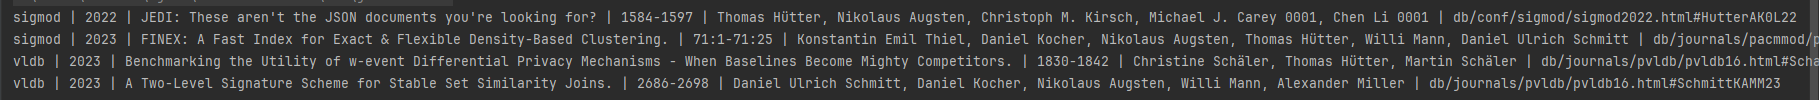
\includegraphics[width=\linewidth]{console.png}
    \caption{Consolenoutput der geparsten Daten}\label{fig:figure}
\end{figure}

\newpage
Geben Sie die Definition Ihrer Tabellen im Edge Modell an. Zeigen Sie (einen Ausschnitt) des Toy Beispiels nach dem Import als Edge Model in die DB (1 P).

\begin{lstlisting}[style=dmrsql]
CREATE TABLE node
    (id SERIAL PRIMARY KEY,s_id TEXT, type TEXT, content TEXT)

CREATE TABLE edge (parents INT, childs INT)
\end{lstlisting}

\begin{figure}[H]
    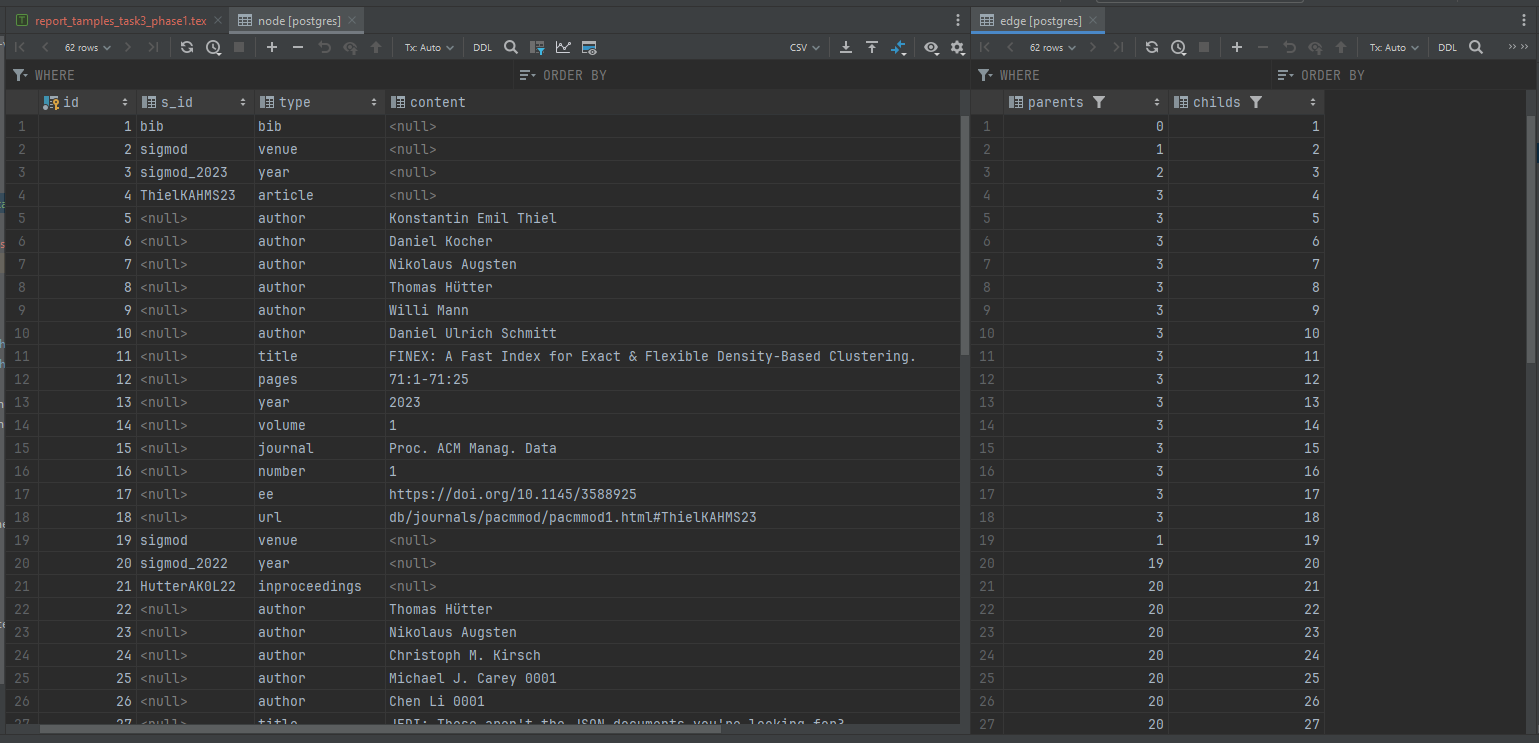
\includegraphics[width=\linewidth]{ausschnitt_node_table.png}
    \caption{Ausschnitt der Node und Edge Table als Edge Modell}\label{fig:node}
\end{figure}

\subsection*{Berechnung der XPath Achsen im EDGE Modell (2 Punkte)}

Geben Sie für jede der geforderten Achsen, die Knotenmenge des Ergebnisses, sowie die Anzahl der Ergebnisknoten aus.

\begin{table}[h]
	\centering
		\begin{center}
			\begin{tabular}{ l | c c }
				\toprule
				Achse & Ergebnisknoten ID's & Ergebnisgröße\\
				\midrule
				ancestor & \{48, 34, 33, 0\} & 4 \\
				descendants & \{35, 36, 37, 38, ..., 62\} & 28 \\
				following SchmittKAMM23 & \emptyset   & 0 \\
				preceeding SchmittKAMM23 & \{35\} & 1 \\
				following SchalerHS23 & \{48\} & 1 \\
				preceeding SchalerHS23 & \emptyset & 0 \\
				\bottomrule
			\end{tabular}
			\end{center}
	\caption{Ergebnisse der XPath-Berechnug}
	\label{tab:ErgebnisseDerXPathBerechnug}
\end{table}

Sofern Sie Annahmen zum Aufbau der Daten getroffen haben, geben Sie diese nachfolgend an:
\begin{itemize}
	\item Annahme 1: Ancestor gibt alle Knoten von der Wurzel aus bis zum gesuchten Knoten.
    \item Annahme 2: Descendants macht genau des umgekehrte und gibt alle Unterknoten vom gewählten Knoten aus, bis zum nächsten Übernknoten.
    \item Annahme 3: following gibt alle Unterknoten des gewählten Überknoten aus.
    \item Annahme 4: preceeding gibt alle vorherigen Knoten des gewählten Knotens aus.
    \item Annahme 5: siehe Phase 2 $->$ Verwendung aus der DBLP, die Präfixe wurden bereits spezifiziert.
    \item Annahme 6: Sortierung selbst: Erst Venue absteigend, dann das Jahr absteigend und anschließend Publikationen absteigend.
\end{itemize}

\subsection*{Verbesserungen & Anpassungen wie verlangt}
Die Tabelle wurde nun soweit angepasst, dass durch die Funktionen preceeding/following/ancestor/descendants die gewollten Werte herauskommen.
\begin{figure}[H]
    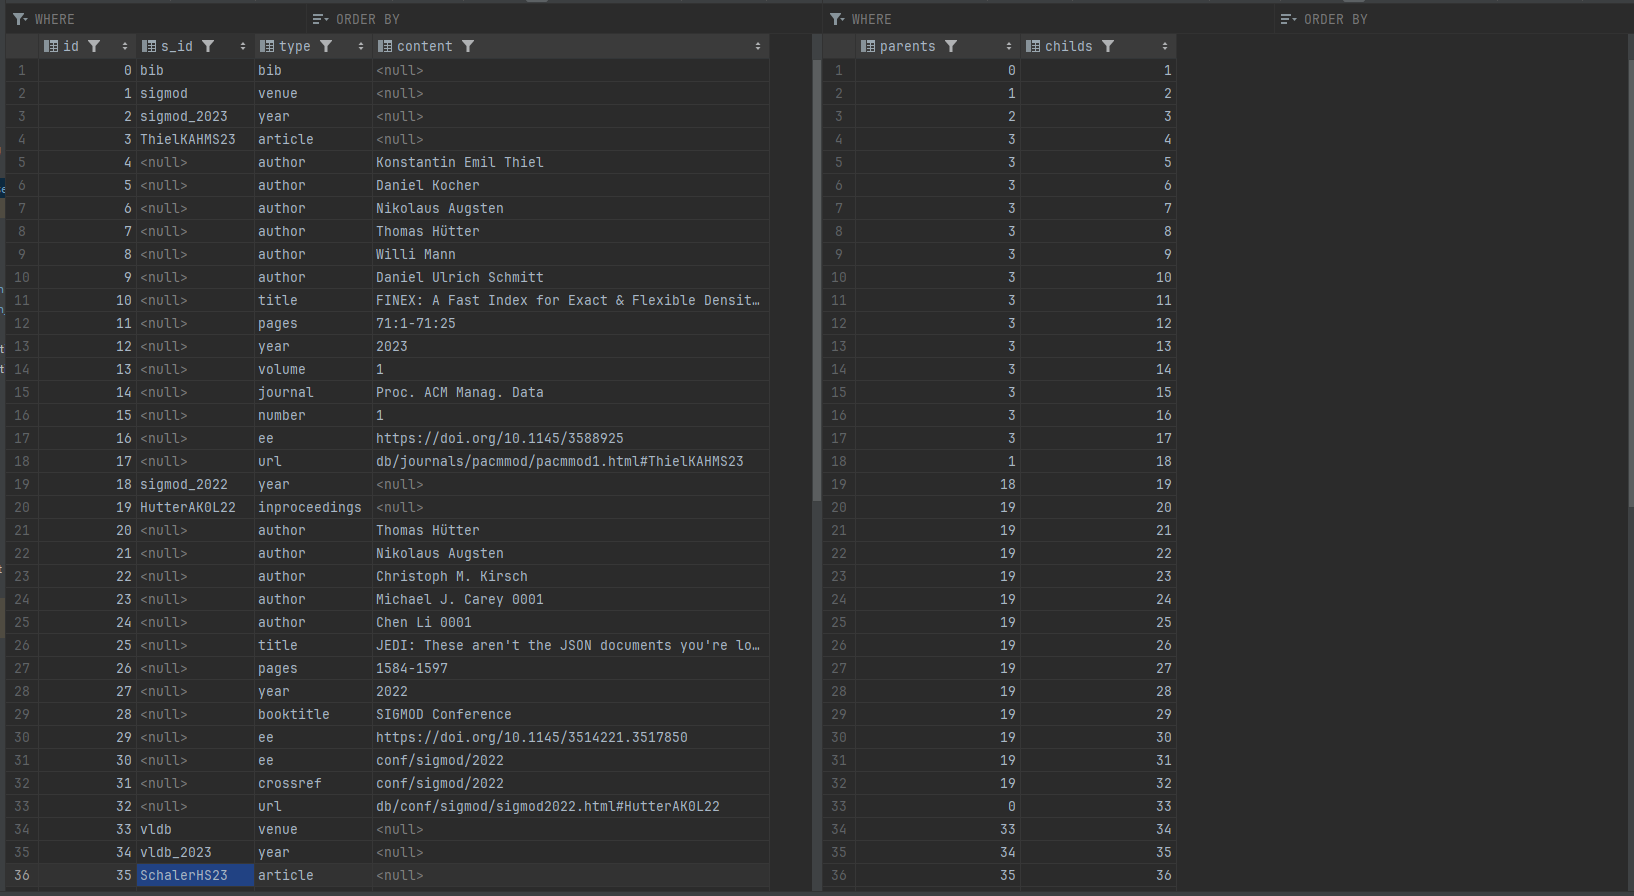
\includegraphics[width=\linewidth]{Verbesserung_Node_Edge_Table.png}
    \caption{Verbesserung der Node/Edge Tabelle Part 1}\label{fig:figure2}
\end{figure}
\begin{figure}[H]
    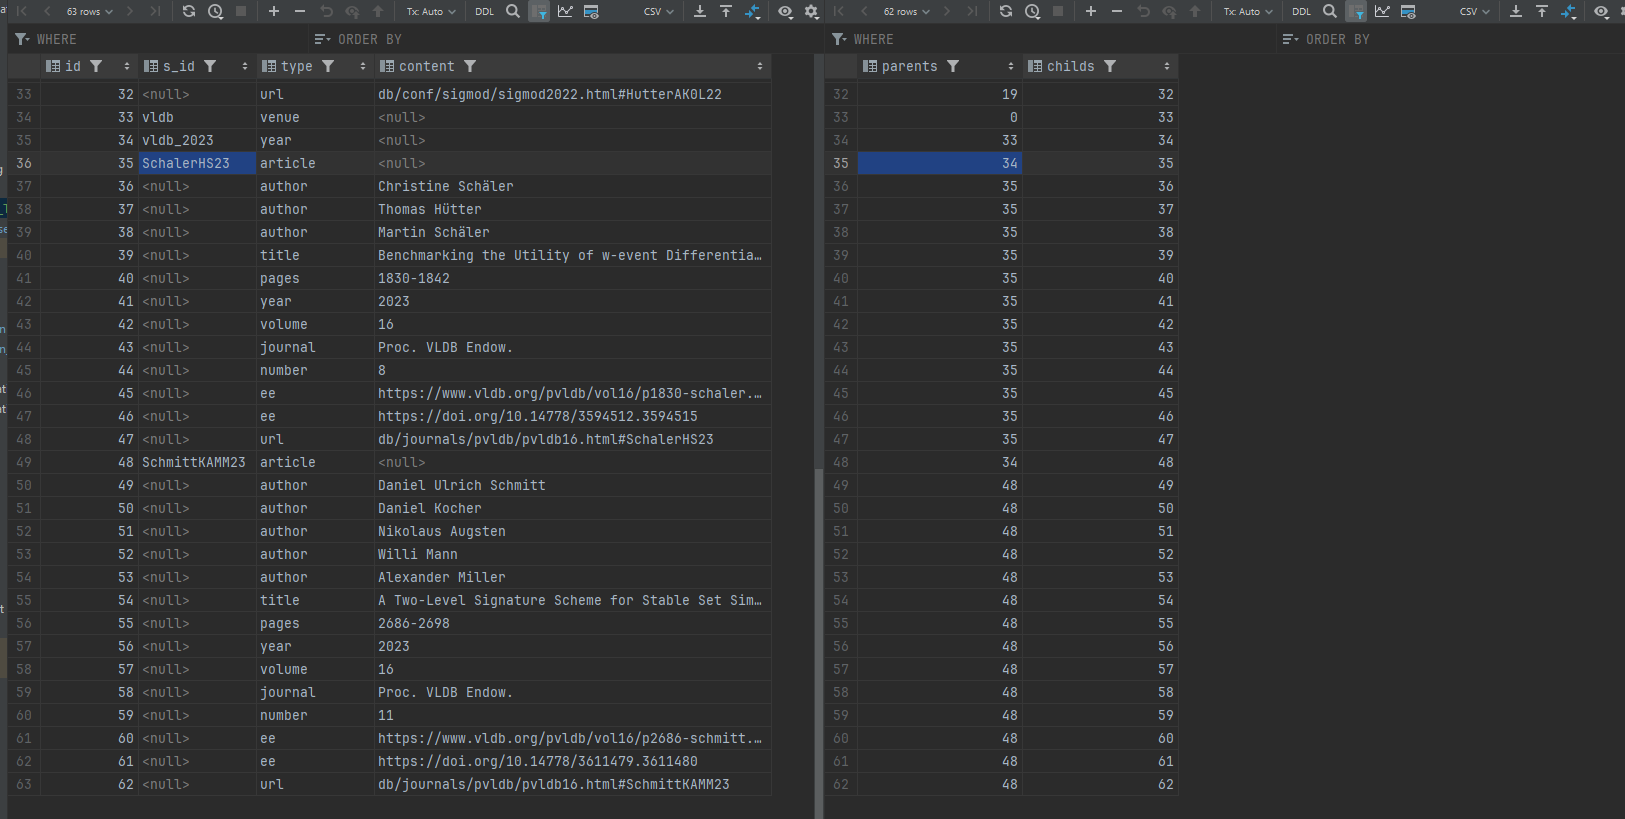
\includegraphics[width=\linewidth]{Verbesserung_Node_Edge_Table_P2.png}
    \caption{Verbesserung der Node/Edge Tabelle Part 2}\\label{fig:figure3}
\end{figure}

\begin{figure}[H]
    \begin{minipage}[b]{.4\linewidth}
        \begin{center}
            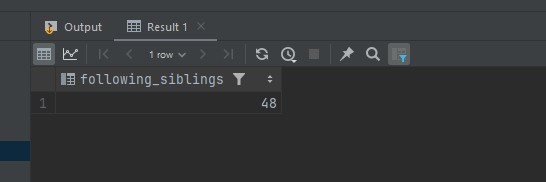
\includegraphics[width=\linewidth]{img.png}
            \caption{Following mit der Value von SchmittKAMM23}
        \end{center}
    \end{minipage}
    \hspace{.1\linewidth}
    \begin{minipage}[b]{.4\linewidth}
        \begin{center}
            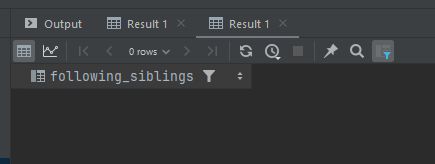
\includegraphics[width=\linewidth]{img_5.png}
            \caption{Following mit der Value of SchalerHS23}
        \end{center}
    \end{minipage}
\end{figure}

\begin{figure}[H]
    \begin{minipage}[b]{.4\linewidth}
        \begin{center}
            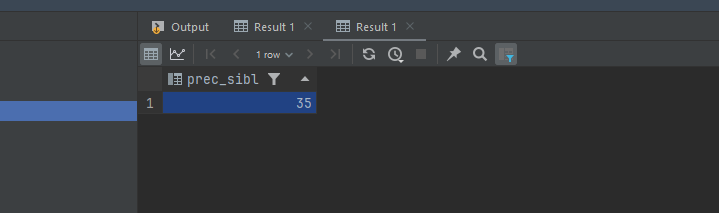
\includegraphics[width=\linewidth]{img_1.png}
            \caption{Preceding mit der Value von SchmittKAMM23}
        \end{center}
    \end{minipage}
    \hspace{.1\linewidth}
    \begin{minipage}[b]{.4\linewidth}
        \begin{center}
            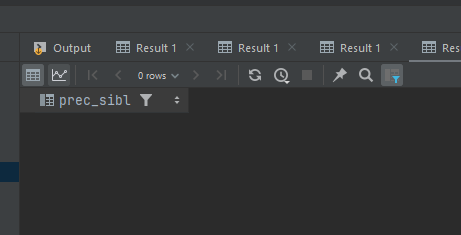
\includegraphics[width=\linewidth]{img_4.png}
            \caption{Preceding mit der Value of SchalerHS23}
        \end{center}
    \end{minipage}
\end{figure}

\begin{figure}[H]
    \begin{minipage}[b]{.4\linewidth}
        \begin{center}
            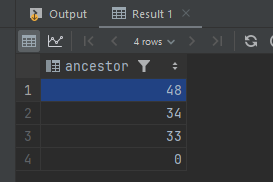
\includegraphics[width=\linewidth]{img_2.png}
            \caption{Ancestors mit dem Value von Daniel Ulrich Schmitt auf ID 49}
        \end{center}
    \end{minipage}
    \hspace{.1\linewidth}
    \begin{minipage}[b]{.4\linewidth}
        \begin{center}
            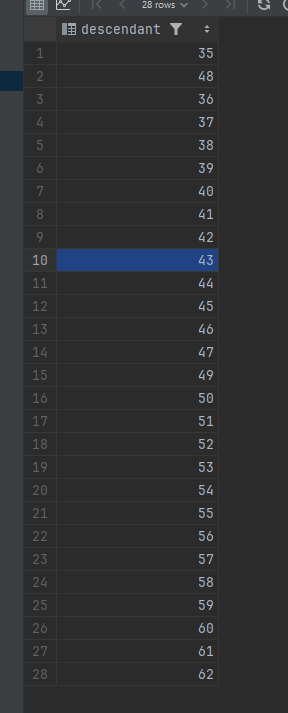
\includegraphics[width=\linewidth]{img_3.png}
            \caption{Descendants von vldb_2023 auf Node 34}
        \end{center}
    \end{minipage}
\end{figure}

\subsection*{Zeitmamagement}

Benötigte Zeit pro Person (nur Phase 1):
\textbf{Alexander Weilert: 9h} \\
\textbf{Dragana Jovanovic: 8h}

\end{document}
